% This is LLNCS.DEM the demonstration file of
% the LaTeX macro package from Springer-Verlag
% for Lecture Notes in Computer Science,
% version 2.4 for LaTeX2e as of 16. April 2010
\documentclass{llncs}

\usepackage[cmex10]{amsmath}
\usepackage{amssymb, amsfonts}

%\usepackage{natbib}
\usepackage{array,multirow}
\usepackage{color, colortbl}
\usepackage{makeidx}  
\usepackage{rotating}
\usepackage{graphicx}

\definecolor{col1}{rgb}{0.988,0.839,0.571}
\definecolor{col2}{rgb}{0.886,0.886,0.555}
\definecolor{col3}{rgb}{0.582,0.661,0.976}
\definecolor{white}{rgb}{1,1,1}

\graphicspath{{./Figures/},{./Figures/OasisCor/},{./Figures/OasisRegression/},{./Figures/Ellipse/}}
\DeclareGraphicsExtensions{.pdf,.png}



\newcommand{\cost}[0]{\mathtt{c}}
\newcommand{\couplingcost}[0]{\mathtt{cost}}
\newcommand{\coupling}[0]{\pi}
\newcommand{\couplings}[0]{\mathcal{C}}
\def\argmin{\mathop{\rm argmin}}
\newcommand{\dimX}{\mathtt{d}}
\newcommand{\Xsp}{{\mathbf{X}}}
\newcommand{\Ysp}{{\mathbf{Y}}}
\newcommand{\lambdaX}{\lambda^\Xsp}
\newcommand{\lambdaY}{\lambda^\Ysp}
\newcommand{\Cjk}{C_{j,k}}
\newcommand{\CjkX}{C^\Xsp_{j,k}}
\newcommand{\CjkY}{C^\Ysp_{j,k}}
\newcommand{\psijkX}{\psi^\Xsp_{j,k}}
\newcommand{\psijkY}{\psi^\Ysp_{j,k}}
\begin{document}

\title{Exploratory Population Analysis with Unbalanced Optimal Transport}
\titlerunning{Exploratory Population Analysis with Unbalanced Optimal Transport}  

\author{Samuel Gerber$^1$, Marc Niethammer$^2$, Martin Styner$^2$, Stephen Aylward$^1$}
\authorrunning{Gerber et al.} 
\institute{Kitware Inc, Carborro NC 27510, USA,
\and
University of North Carolina, Chapel Hill NC 27504, USA\\
\email{samuel.gerber@kitware.com}
}


\maketitle              

\begin{abstract}
The plethora of data from neuroimaging studies provide a rich opportunity to
discover effects and generate hypotheses through exploratory data analysis.
Brain pathologies often manifest in changes in shape along with deterioration
and alteration of brain matter, i.e., changes in mass. We propose a morphometry
approach using unbalanced optimal transport that detects and localizes changes in
mass and separates them from changes due to the location of mass. The approach
generates images of mass allocation and mass transport cost for each subject in
the population. Voxelwise correlations with clinical variables highlights
regions of mass allocation or mass transfer related to the variable.  We
demonstrate the method on the white and gray matter segmentations
from the OASIS brain MRI data set.  The separation of white and gray matter
ensures that optimal transport does not transfer mass between different
tissues types and separates gray and white matter related changes. The OASIS
data set includes subjects ranging from healthy to mild and moderate dementia,
and the results corroborate known pathology changes related to dementia that
are not discovered with traditional voxel-based morphometry. The
transport-based morphometry increases the explanatory power of regression on
clinical variables compared to traditional voxel-based morphometry, indicating
that transport cost and mass allocation images capture a larger portion of
pathology induced changes.  
\end{abstract}



\section{Introduction}
Neurological disease and disorder manifest in subtle and varied changes in
brain anatomy that can be non-local in nature and effect amounts of white and
gray matter as well as relative positioning and shapes of local brain anatomy.
To detect and quantify these changes is a primary goal of morphometry based
population analysis. We propose a morphometry approach based on unbalanced
optimal transport, termed UTM, that yields a voxelwise comparison but can
detect global and regional deterioration of matter. The UTM formulation
explicitly separates changes in matter volume from changes in matter location.
This separation of effects leads to stronger correlations and more readily
interpretable visualizations. 

Optimal transport, as the name implies, solves the problem of transporting mass
from a probability measure $\mu$ to a probability measure $\nu$, such that the
cost of moving mass from the source $\mu$ to the target $\nu$ is minimized.
Unbalanced optimal transport~\cite{guittet2002extended,benamou2003numerical}
extends optimal transport to measures that do not need to have equal mass by
adding a mechanism to add mass to the optimization problem. The solution of the
unbalanced optimal transport yields a transport plan, or coupling, that
measures local mass allocation and movement between source and target
locations. We decompose these transport plans to measure for each subject, at
each voxel, mass allocations and costs of mass transfer. These two measures
explicitly separate changes due to differences in amount of matter from
differences due to changes in location of matter related to relative position
and shape of anatomies. 

Voxel-based morphometry (VBM)~\cite{ashburner2000voxel} yields spatially
localized changes in brain anatomy but has difficulty in discovering regionally
or globally occurring changes. Figure~\ref{fig:cor-ellipse} demonstrate the
capability of UTM to detect changes in size on a toy example of a hundred
half--ellipses with different ellipticity and thickness.  Correlating the
mass allocation and mass transfer images from UTM with either shape or size of
the half--ellipses shows that the proposed method is capable of correctly
attributing changes to either variation in shape or size.  Traditional VBM
results in weak correlation with changes in size and cannot attribute the
source of the changes to ellipse shape or size.

\begin{figure}[t!]
\scriptsize
\centering
%\begin{tabular}{l}
\begin{tabular}{ll}
\begin{tabular}{lccc}
  \raisebox{2.5mm}{\rotatebox[origin=c]{90}{ $ \longrightarrow $ } }&
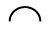
\includegraphics[width=0.11\linewidth]{illustration-01-01} &
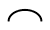
\includegraphics[width=0.11\linewidth]{illustration-02-01} &
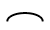
\includegraphics[width=0.11\linewidth]{illustration-03-01} \\
  \raisebox{2.5mm}{\rotatebox[origin=c]{90}{ Size } }&
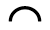
\includegraphics[width=0.11\linewidth]{illustration-01-02} &
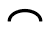
\includegraphics[width=0.11\linewidth]{illustration-02-02} &
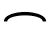
\includegraphics[width=0.11\linewidth]{illustration-03-02} \\
  \raisebox{2.5mm}{\rotatebox[origin=c]{90}{ $ \longleftarrow $ }} &
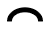
\includegraphics[width=0.11\linewidth]{illustration-01-03} &
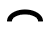
\includegraphics[width=0.11\linewidth]{illustration-02-03} &
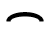
\includegraphics[width=0.11\linewidth]{illustration-03-03} \\
  & $ \longleftarrow $ & Shape & $ \longrightarrow $ \\
\end{tabular}
        &
\begin{tabular}{r}
\begin{tabular}{lrcr}
 Pearson's r  &-0.9 & 
\includegraphics[width=0.3\linewidth]{colorbar} & 0.9
\end{tabular}\\
\begin{tabular}{rl|ccc}
%\rowcolor{col3}\\ 
        \hline 
  \rotatebox[origin=c]{90}{ VBM} & &
  \raisebox{-3mm}{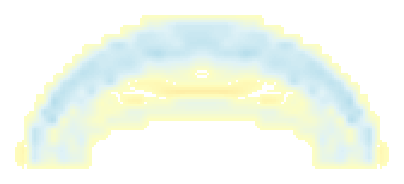
\includegraphics[width=0.155\linewidth]{cor-mass-intensity}} &
  \raisebox{-3mm}{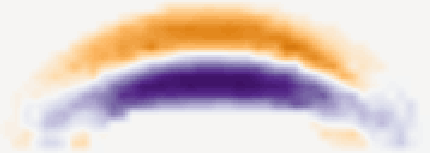
\includegraphics[width=0.155\linewidth]{cor-rx-ry-intensity} }&
  \raisebox{-3mm}{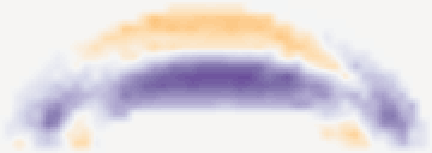
\includegraphics[width=0.155\linewidth]{cor-rx-ry-mass-intensity}} \\ 
  \hline
  \hline
%\rowcolor{col1}
  \raisebox{2mm}{ \multirow{2}{1.5mm}{ \rotatebox[origin=c]{90}{UTM} }} &
  \raisebox{1mm}{\rotatebox[origin=c]{90}{Cost}}&
  \raisebox{-2mm}{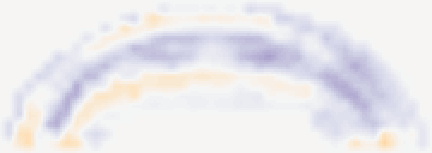
\includegraphics[width=0.155\linewidth]{cor-mass-cost} }&
  \raisebox{-2mm}{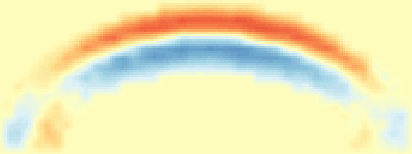
\includegraphics[width=0.155\linewidth]{cor-rx-ry-cost} }&
  \raisebox{-2mm}{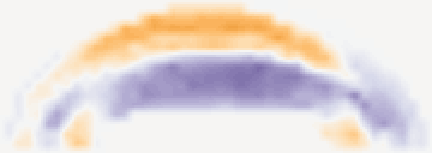
\includegraphics[width=0.155\linewidth]{cor-rx-ry-mass-cost} } \\
  %
  &
  \raisebox{1mm}{\rotatebox[origin=c]{90}{Mass}}&
  \raisebox{-2mm}{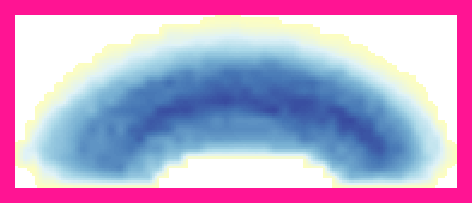
\includegraphics[width=0.155\linewidth]{cor-mass-mass-border} }&
  \raisebox{-2mm}{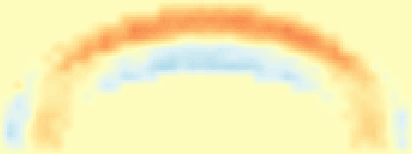
\includegraphics[width=0.155\linewidth]{cor-rx-ry-mass} }&
  \raisebox{-2mm}{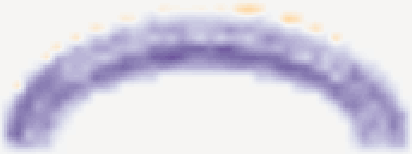
\includegraphics[width=0.155\linewidth]{cor-rx-ry-mass-mass} }\\ \hline 
%\rowcolor{white}
  &
  & cor( Size ) 
  & cor( Shape )
  & cor( Shape + Size)
\end{tabular}\\
\end{tabular}\\
  (I) & (II) \\
\end{tabular}
%\begin{tabular}{c|c|c|r}
%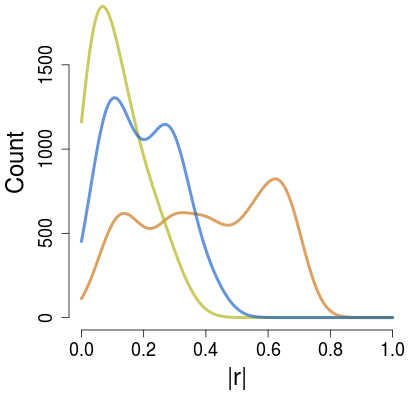
\includegraphics[width=0.25\linewidth]{hist-mass} &
%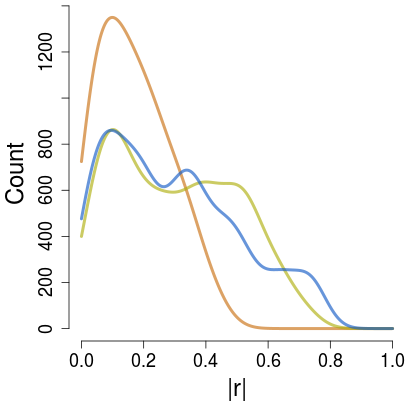
\includegraphics[width=0.25\linewidth]{hist-ellipticity} &
%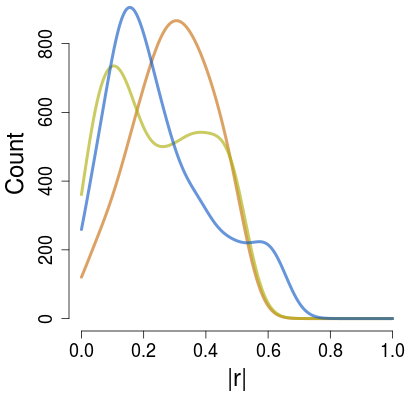
\includegraphics[width=0.25\linewidth]{hist-additive} &
%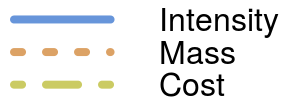
\includegraphics[width=0.15\linewidth]{legend} 
%  \\ \hline 
%	(a') Size & (b') Shape & (c') Shape + Size &
%\end{tabular}\\
%  (III)
%\end{tabular}
\caption{\label{fig:cor-ellipse}
(I) Illustration of unbalanced optimal transport on a toy data set of a 100
half--ellipses with different shapes (ratio of major to minor radius) and sizes
(black pixel count).  (II) Spatial correlations of size, shape and
size + shape to VBM (pixel intensity) and UTM (mass allocation
and transport costs).  Positive and negative correlation indicate an
increase and decrease of mass, cost, or intensity, respectively. Only UTM is
able to detect size variation (highlighted box) as strongly positively
correlated to mass allocation.  Both UTM and VMB detect shape variation,
with stronger correlations in transport cost than mass allocation in UTM. UTM
identifies both change in shape and mass for the variable depending on shape
plus size. 
%(III) Smoothed counts of Pearson's r correlation from the spatial
%correlations. The proposed method correctly identifies shape versus mass
%effects and leads to stronger correlations.  
\vspace{-7mm}
}
\end{figure}

Deformation-based morphometry (DBM)~\cite{ashburner1998identifying} addresses
the issue of detecting global effects by comparing the parameters of non-linear
spatial normalizations to a template.  DBM results, typically shown as modes of
variation, are more difficult to visualize and interpret.  UTM combines the
strengths of VBM and DBM methods.  While the results are based on a voxelwise
analysis and easily interpretable, the quantities compared stem from a global
optimization problem which can detect global and regional effects.  

A key observation is that VBM, TBM and DBM are driven by local image gradients
and voxelwise measures ultimately lead to very similar
results~\cite[Chaper~6]{frackowiak2004human}.  UTM solves a global optimization
problem based on the distribution of mass and the allocation of mass is not
driven by image gradients. In UTM allocation of mass can be diffuse over a
large region without the need for a smooth spatial normalization to distribute
the image gradient driven warp over a larger region. 

VBM has been shown to be sensitive to the particulars of the spatial
normalization~\cite{bookstein2001voxel,davatzikos2004voxel}. UTM still depends
on a rigid spatial normalization to bring the subjects into a common coordinate
system were voxelwise comparisons are feasible. However, the optimal transport
is insensitive to small miss-alignments in the spatial normalization step;
small shifts in mass locations incur only small transport costs.  After the
spatial normalization UTM does not depend on a template, the mass allocation
and transport cost images are based on an averaging of quantities derived from
pairwise transport plans, which alleviates bias due to registrations to a
single template. 

The key contributions of this work are:
\vspace{-1mm}
\begin{enumerate}
\item A voxel-wise morphometry approach capable of detecting regional and
  global changes.  
\item A formulation of unbalanced optimal transport to detect and disentangle mass
  changes 
\item A demonstration of the importance of incorporating mass imbalances to
  detect and localize neurodegenerative anatomical changes.
  (Section~\ref{sec:results}).from changes in mass location (Section~\ref{sec:methods}).
\item An application of optimal transport to gray and white matter masks
  individually to avoid mass exchange between tissues and incommensurable
  measurements across subjects in MRI intensities (Section~\ref{sec:results}).  
\end{enumerate}


\section{Related Work}
Recent advances in the computation of optimal transport
plans~\cite{cuturi2013sinkhorn,gerber2017multiscale} paved the way for a flurry
of applications in machine learning and spurred interest in applications to
medical image analysis. Gramfort et.  al.~\cite{gramfort2015fast} use optimal
transport for improved averaging of neuroimaging data, Feydy et
al.~\cite{feydy2017optimal} use unbalanced optimal transport as a similarity
measure for diffeomorphic registration and Kundu et.
al.~\cite{kundu2018discovery} formulate a DBM approach, TrBM, which replaces
non-linear warps by optimal transport plans. 

UTM integrates optimal transport to morphometric analysis in a different way
from TrBM.  TrBM yields a parametrization of the transport plans akin to DBM
that captures global changes. UTM uses the transport plan to create voxelwise
measures and adds mass imbalances into the transport plans, which prove to be
an important indicator in neurodegenerative diseases.  The TrBM is applied to
graylevel MRI intensities, we choose to use the gray and white matter masks
instead of MRI intensity values to avoid conversion of white to gray matter in
the optimal transport optimization and to avoid difficulties in normalizing MRI
intensities across subjects. 


\section{Unbalanced Optimal Transport Morphometry}
\label{sec:methods}
Morphometry with unbalanced optimal transport follows the standard voxelwise
morphometry pipeline but performs voxelwise statistical analysis on the mass
allocation and transport cost images derived from the solution of unbalanced
optimal transport between the subjects. Section~\ref{sec:unbalanced} describes
the unbalanced optimal transport problem and Section~\ref{sec:mass} the
construction of the mass allocation and transport cost maps for each subject.

\subsection{Unbalanced Optimal Transport}
\label{sec:unbalanced}
For two probability measures $\mu$ and $\nu$ on probability spaces ${\Xsp}$
and ${\Ysp}$ respectively, a coupling of $\mu$ and $\nu$ is a measure
$\coupling$ on ${\Xsp}\times{\Ysp}$ such that the marginals of $\coupling$ are
$\mu$ and $\nu$. The coupling $\coupling$ defines a {\em transport plan} that
captures how much mass $\coupling(x, y)$ is transported from any $x \in \Xsp$
to any $y \in \Ysp$. To define optimal transport and optimal couplings, we need
a cost function $\cost(x,y)$ on ${\Xsp}\times{\Ysp}$ representing the work or
cost needed to move a unit of mass from $x$ to $y$. An optimal coupling
$\coupling^*$ minimizes this cost over all choices of couplings
$\mathcal{C}(\mu,\nu)$ between
$\mu$ and $\nu$: 
\begin{equation}
  \coupling^*= \argmin_{\coupling\in\mathcal{C}(\mu,\nu)} \int_{{\Xsp}}\int_{{\Ysp}}
\cost(x,y)  d\coupling(x,y) \,.  
\end{equation}

For discrete distributions $\mu = \sum_1^n w(x_i) \delta(x_i)$ and $ \nu =
\sum_1^m v(y_i) \delta(y_i)$ with $\sum w(x_i) = \sum v(y_i) = 1$ the optimal
transport problem can be solved by linear programming. To extend the
formulation to deal with arbitrary positive measures $\mu$ and $\nu$ with mass
imbalance  $\Delta = \lvert \sum_1^n v(y_i)  - \sum_1^m w(x_i) \rvert$, the
linear program is modified to allow for the creation of mass by adding a new
source location $z^s$ and target location $z^t$ and constraints to restrict the
amount of mass added to be at most $w(x_i)$ and $v(x_i)$ at any target and
source location, respectively. With these modifications the linear program reads: 
\begin{equation}
\min_\coupling \sum_{\substack{i=1,\dots,n\\ j=1,\dots,m}} 
      \cost(x_i, y_j) \coupling(x_i, y_j) \, \text{s.t.}\, 
\begin{cases}
  \sum_j \coupling(x_i, y_j) + \coupling(x_i, z^t) = \mu(\{x_i\}) = w(x_i) & \\ 
  \sum_i \coupling(x_i, y_j) + \coupling(z^s, y_j) = \nu(\{y_j\}) = v(y_j) & \\
  \sum_j \coupling(x_i, z^t) + \sum_j \coupling(z^s, y_j)  = \Delta \\
  \coupling(x_i, y_j) \ge 0 \,, \coupling(z^s, y_j) \ge 0 \,, \coupling(x_i,
  z^t) \ge 0  \\
\end{cases}
\label{eq:unbalanced}
\end{equation} 

The modifications result in a standard optimal transport problem that can, with
only minor modifications, be solved by fast approximation algorithms for large
data sets such as the Sinkhorn approach~\cite{cuturi2013sinkhorn} or multiscale
strategies~\cite{gerber2017multiscale}. 

An arbitrary cost $\cost(x^s, y_j)$ and  $\cost(x_i, y^t)$ can be assigned
to allocate mass, and restriction to only allocate $\Delta$ amount of mass can
be relaxed or removed, striking a trade-off between the cost of creating mass
and the cost of moving mass. For our application, we choose the allocation of
mass at zero cost but only allow for the allocation of exactly $\Delta$ mass.
This forces the transfer of all jointly available mass between source and
target location and distribute the mass $\Delta$ optimally to reduce the cost
of movement.

Solving the unbalanced optimal transport problem is convex and yields a global
minimum without any parameter tuning, the only choice is the selection of a
cost $\cost$.

\subsection{Construction of Mass Allocation and Transport Cost Images}
\label{sec:mass}
For an image $X^k$ denote by $X^k(x_i)$ the associated non-negative value at
voxel location $x_i$, which defines a measure $\mu^k = \sum_1^n X^k(x_i)
\delta(x_i)$.  To construct the voxelwise mass allocation and transport cost
images we solve for optimal transport plans $\coupling^*_{k,l}$ between all
images $X^k$ and $X^l$.  The variables $z^s$ and $z^t$ in
equation~\ref{eq:unbalanced} capture the amount of mass allocated when moving
mass from $X^k$ to $X^l$. Denote by $z^s_{k, l}$ and $z^t_{k,l}$ the mass
allocation variable associated with the optimal transport plan
$\coupling^*_{k,l}$. For subject $X_k$ the mass allocation image $M^k$ is
constructed by 
$
M^k(x_i) = \sum_l \left( 
  \coupling^*_{k,l}( z^s_{k, l}, x_i) - 
  \coupling^*_{k,l}( x_i, z^t_{k, l} ) 
\right)
$ 
and the transport cost image by 
$C^k(x_i) = \sum_l \sum_j \coupling^*_{k,l}( x_i, x_j ) \cost(x_i, y_j)$

The images $M^k$ and $C^k$ are smoothed with a small Gaussian to increase
correlations between neighboring pixels. The smoothed images $M^k$ and $C^k$
replace the smoothed intensity or Jacobian determinant images in the
statistical analysis of a VBM or TBM pipeline. 


\section{Application to OASIS Brain MRI}
\label{sec:results}
We apply UTM to the OASIS brain data set~\cite{marcus2010open}. Code to
replicate the results is located at
\url{https://github.com/KitwareMedical/UTM}. The OASIS database consists of T1
weighted MRI of 416 subjects aged 18 to 96.  One hundred of the subjects over
the age of 60 are diagnosed with mild to moderate dementia. The images in the
OASIS data set are already skull-stripped, gain-field corrected and registered
to the Talaraich atlas space~\cite{talaraich:book88} with a 12-parameter affine
transform.  To focus on dementia related effects we restrict the analysis to
137 patients from age 60 to 80. This set of patients contains 66 healthy
patents and 71 patients with a diagnosis of very mild to moderate dementia as
established by a clinical dementia rating (CDR, 0 = normal, 0.5 = very mild, 1
= Mild, 2 = Moderate ). In addition to CDR the data set contains information
about Age and a mini mental state examination score (MMSE, count of correct
answers with a perfect score of 30).

\begingroup
\renewcommand{\arraystretch}{0}
\setlength{\tabcolsep}{0pt}
\begin{figure}[!h]
\scriptsize
\centering
\begin{tabular}{r}
\begin{tabular}{lrcr}
  \parbox[t][3mm]{20mm}{Pearson's r}&
  \parbox[t][3mm]{7mm}{-0.7} & 
  
\includegraphics[width=0.6\linewidth]{colorbar} & 
   \parbox[t][3mm]{6mm}{\hfill 0.7}
\end{tabular}\\
\begin{tabular}{c|cc||cc||cc} 
  \multirow{3}{1mm}{\raisebox{-7mm}{\rotatebox[origin=c]{90}{VBM}} } &
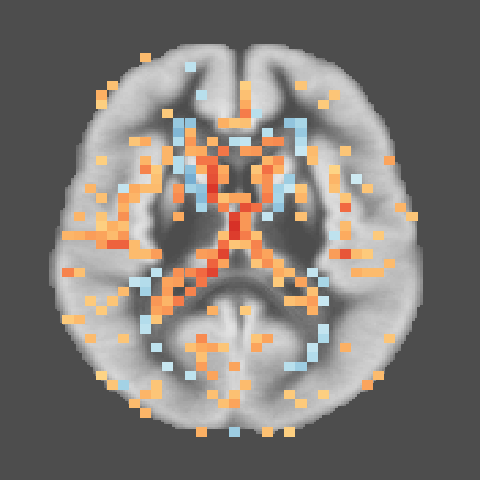
\includegraphics[width=0.146\linewidth]{cor-axial-age-t-iG} &
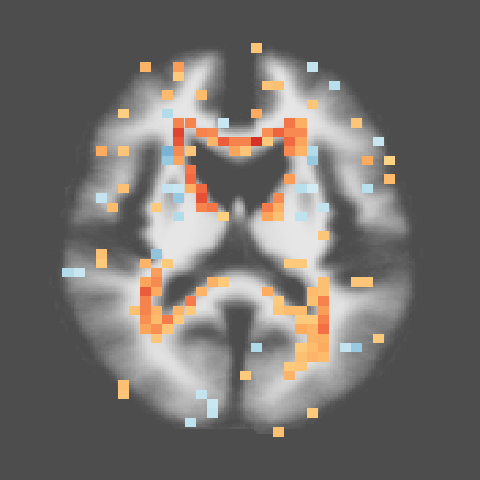
\includegraphics[width=0.146\linewidth]{cor-axial-age-t-iW} &
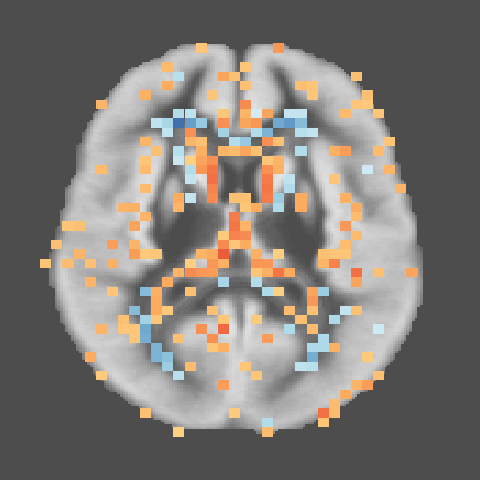
\includegraphics[width=0.146\linewidth]{cor-axial-cdr-t-iG} &
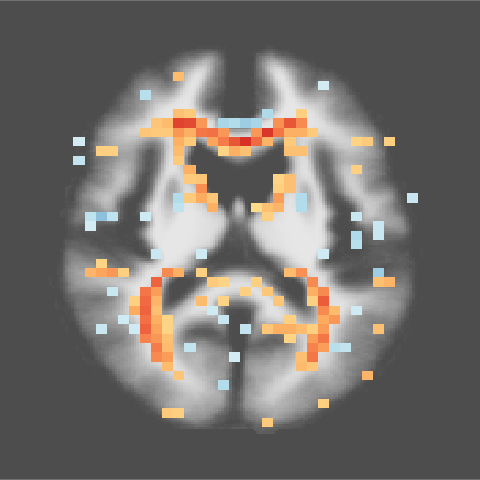
\includegraphics[width=0.146\linewidth]{cor-axial-cdr-t-iW} &
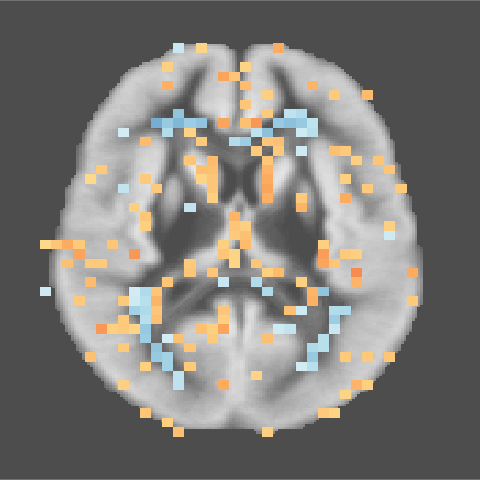
\includegraphics[width=0.146\linewidth]{cor-axial-mmse-t-iG} &
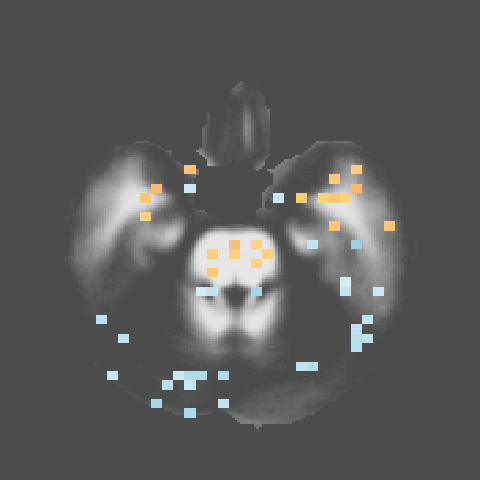
\includegraphics[width=0.146\linewidth]{cor-axial-mmse-t-iW} \\ 
        &
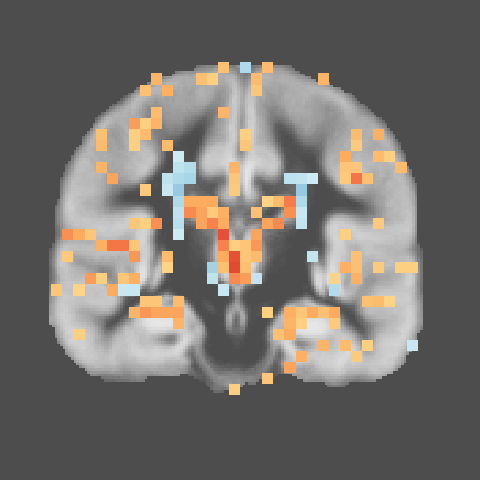
\includegraphics[width=0.146\linewidth]{cor-coronal-age-t-iG} &
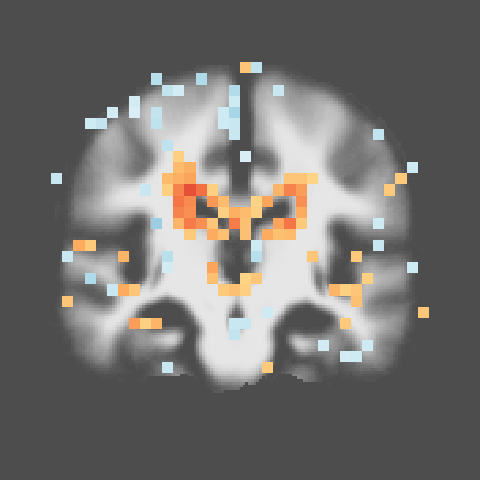
\includegraphics[width=0.146\linewidth]{cor-coronal-age-t-iW} &
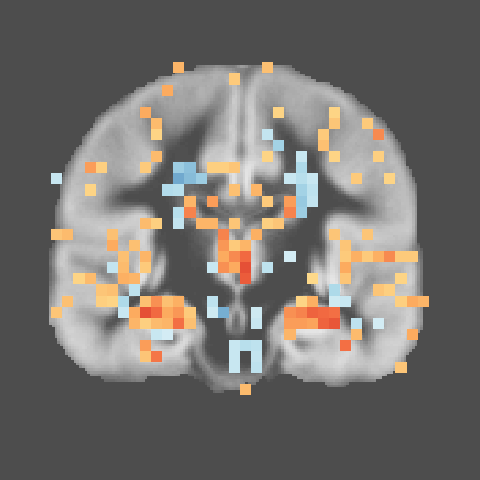
\includegraphics[width=0.146\linewidth]{cor-coronal-cdr-t-iG} &
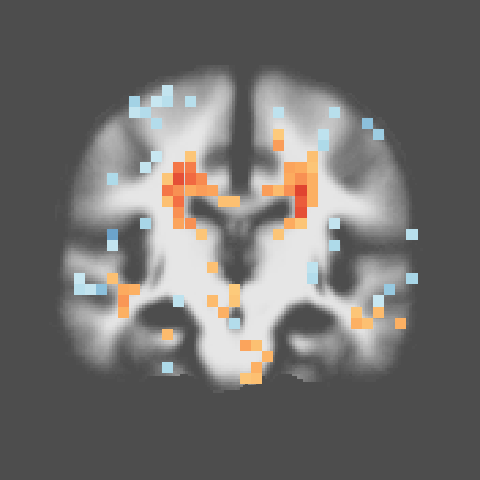
\includegraphics[width=0.146\linewidth]{cor-coronal-cdr-t-iW} &
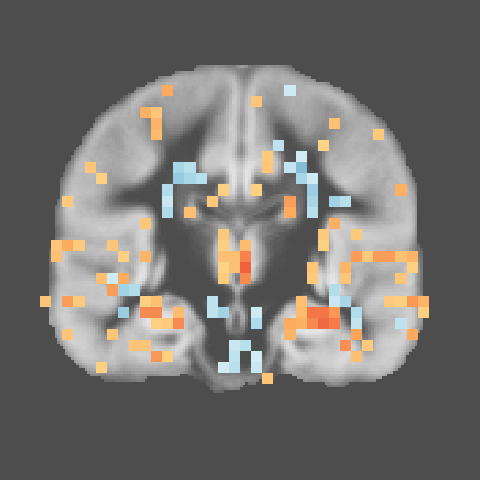
\includegraphics[width=0.146\linewidth]{cor-coronal-mmse-t-iG} &
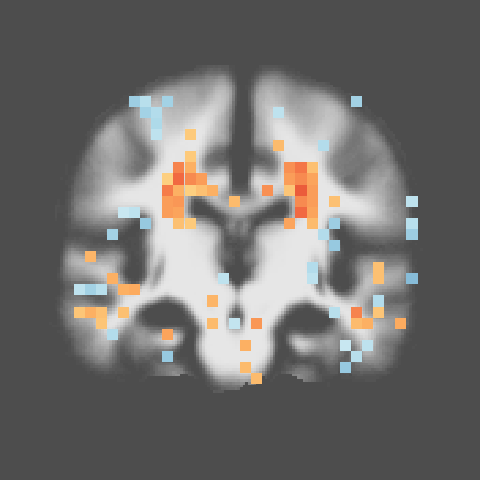
\includegraphics[width=0.146\linewidth]{cor-coronal-mmse-t-iW} \\ 
        &
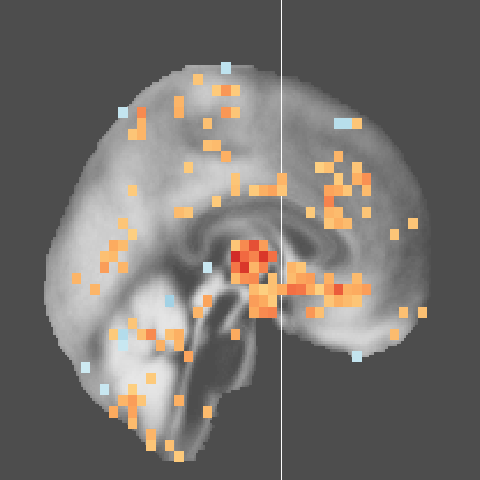
\includegraphics[width=0.146\linewidth]{cor-sagital-age-t-iG} &
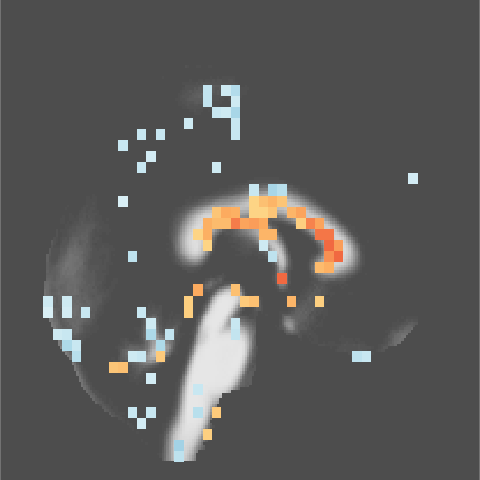
\includegraphics[width=0.146\linewidth]{cor-sagital-age-t-iW} &
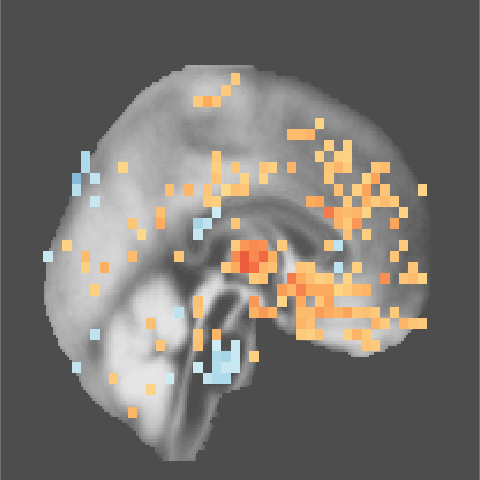
\includegraphics[width=0.146\linewidth]{cor-sagital-cdr-t-iG} &
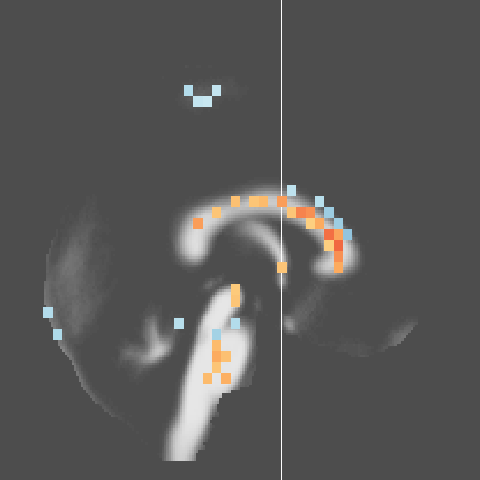
\includegraphics[width=0.146\linewidth]{cor-sagital-cdr-t-iW} &
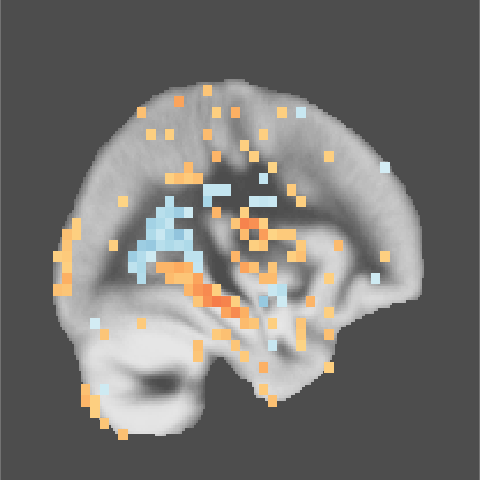
\includegraphics[width=0.146\linewidth]{cor-sagital-mmse-t-iG} &
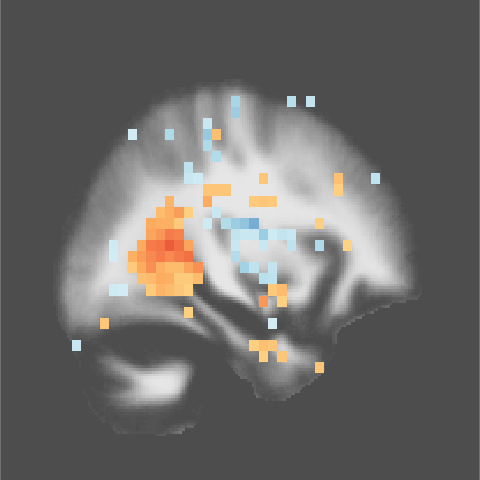
\includegraphics[width=0.146\linewidth]{cor-sagital-mmse-t-iW} \\  
  \hline 
  \hline
    \raisebox{1mm}{ \multirow{3}{2mm}{\rotatebox[origin=c]{90}{UTM Transport Cost}} } &
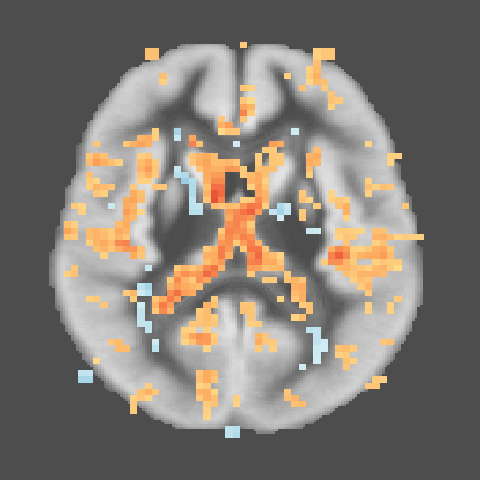
\includegraphics[width=0.146\linewidth]{cor-axial-age-t-tG} &
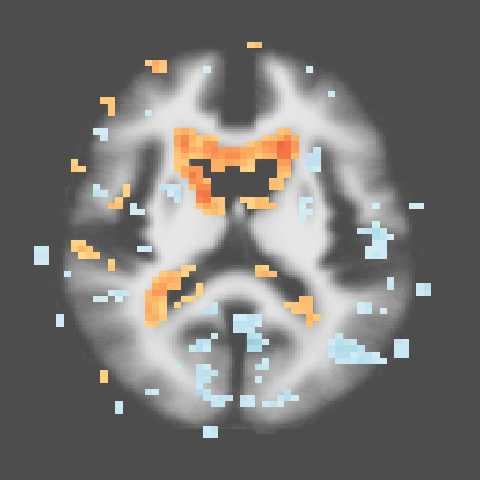
\includegraphics[width=0.146\linewidth]{cor-axial-age-t-tW} &
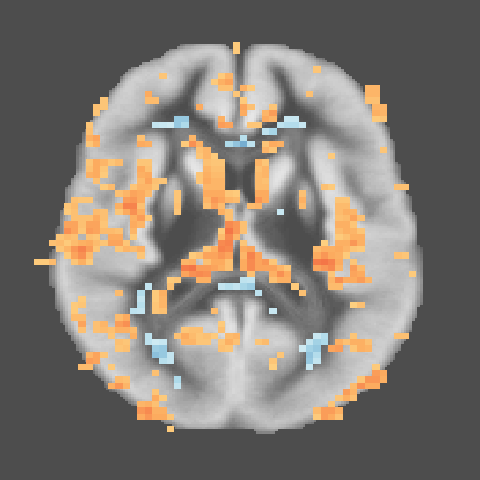
\includegraphics[width=0.146\linewidth]{cor-axial-cdr-t-tG} &
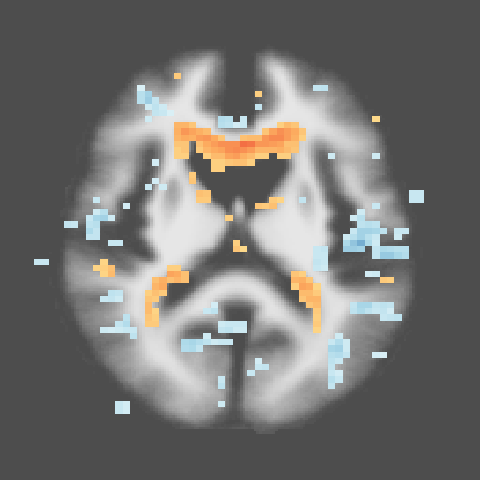
\includegraphics[width=0.146\linewidth]{cor-axial-cdr-t-tW} &
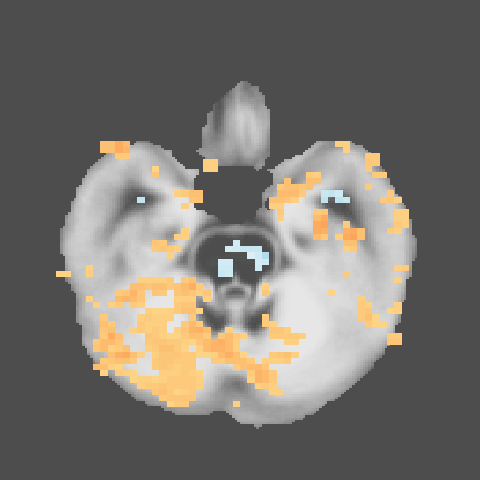
\includegraphics[width=0.146\linewidth]{cor-axial-mmse-t-tG} &
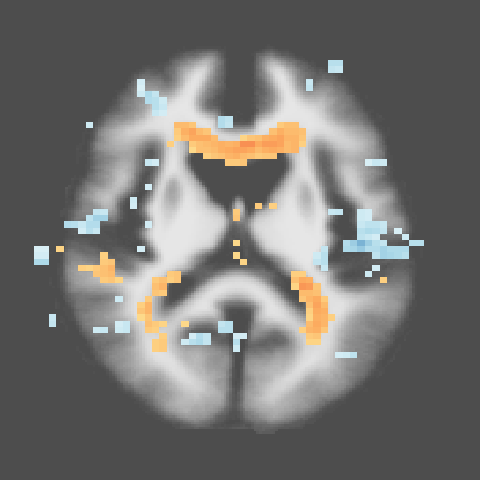
\includegraphics[width=0.146\linewidth]{cor-axial-mmse-t-tW} \\ 
        &
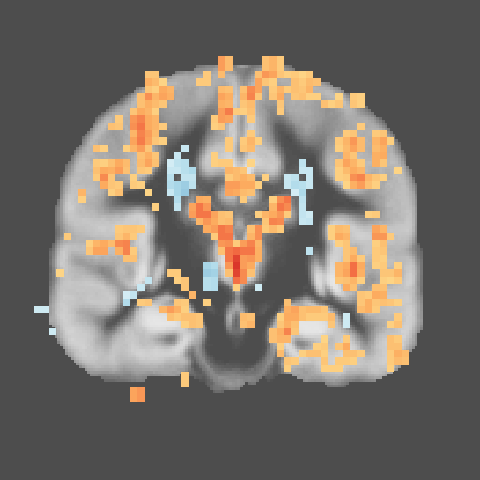
\includegraphics[width=0.146\linewidth]{cor-coronal-age-t-tG} &
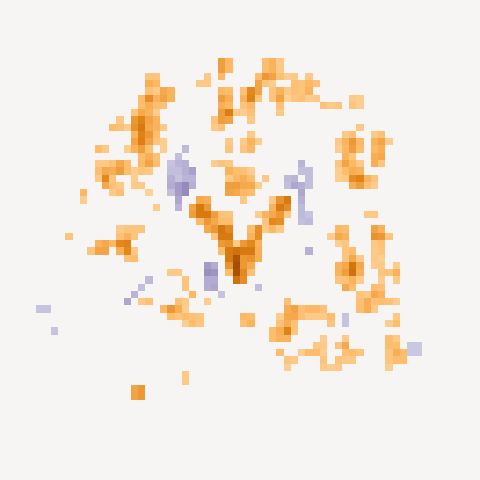
\includegraphics[width=0.146\linewidth]{cor-coronal-age-t-tW} &
\includegraphics[width=0.146\linewidth]{cor-coronal-cdr-t-tG} &
\includegraphics[width=0.146\linewidth]{cor-coronal-cdr-t-tW} &
\includegraphics[width=0.146\linewidth]{cor-coronal-mmse-t-tG} &
\includegraphics[width=0.146\linewidth]{cor-coronal-mmse-t-tW} \\ 
&
\includegraphics[width=0.146\linewidth]{cor-sagital-age-t-tG} &
\includegraphics[width=0.146\linewidth]{cor-sagital-age-t-tW} &
\includegraphics[width=0.146\linewidth]{cor-sagital-cdr-t-tG} &
\includegraphics[width=0.146\linewidth]{cor-sagital-cdr-t-tW} &
\includegraphics[width=0.146\linewidth]{cor-sagital-mmse-t-tG} &
\includegraphics[width=0.146\linewidth]{cor-sagital-mmse-t-tW} \\ 
  \hline 
  \hline
  \raisebox{1mm}{ \multirow{3}{4mm}{ \rotatebox[origin=c]{90}{UTM Mass Allocation} }} &
\includegraphics[width=0.146\linewidth]{cor-axial-age-t-mG} &
\includegraphics[width=0.146\linewidth]{cor-axial-age-t-mW} &
\includegraphics[width=0.146\linewidth]{cor-axial-cdr-t-mG} &
\includegraphics[width=0.146\linewidth]{cor-axial-cdr-t-mW} &
\includegraphics[width=0.146\linewidth]{cor-axial-mmse-t-mG} &
\includegraphics[width=0.146\linewidth]{cor-axial-mmse-t-mW} \\ 
        &
\includegraphics[width=0.146\linewidth]{cor-coronal-age-t-mG} &
\includegraphics[width=0.146\linewidth]{cor-coronal-age-t-mW} &
\includegraphics[width=0.146\linewidth]{cor-coronal-cdr-t-mG} &
\includegraphics[width=0.146\linewidth]{cor-coronal-cdr-t-mW} &
\includegraphics[width=0.146\linewidth]{cor-coronal-mmse-t-mG} &
\includegraphics[width=0.146\linewidth]{cor-coronal-mmse-t-mW} \\ 
        &
\includegraphics[width=0.146\linewidth]{cor-sagital-age-t-mG} &
\includegraphics[width=0.146\linewidth]{cor-sagital-age-t-mW} &
\includegraphics[width=0.146\linewidth]{cor-sagital-cdr-t-mG} &
\includegraphics[width=0.146\linewidth]{cor-sagital-cdr-t-mW} &
\includegraphics[width=0.146\linewidth]{cor-sagital-mmse-t-mG} &
\includegraphics[width=0.146\linewidth]{cor-sagital-mmse-t-mW} \\ 

\hline \hline
& \parbox[b][3mm]{12mm}{Age (g)} 
& \parbox[b][3mm]{12mm}{Age (w)} 
& \parbox[b][3mm]{15mm}{CDR (g)} 
& \parbox[b][3mm]{15mm}{CDR (w) }
& \parbox[b][3mm]{15mm}{-MMSE (g)}
& \parbox[b][3mm]{15mm}{-MMSE (w)}
\end{tabular}
\end{tabular}
\caption{\label{fig:cor-oasis}
Correlation of Age, MMSE and CDR with VBM, UTM mass imbalances and UTM
transport costs on (g) gray and (w) white matter segmentations.  Correlations
are only shown at locations permutation tested p--value less than 0.05 (1000
permutations). The background image are average white and gray matter
segmentations.
\vspace{-4.5mm}
} 
\end{figure} \endgroup
We construct mass allocation and transport cost images for white and gray
matter segmentation masks individually. However, the method can without
modification be applied to any scalar image or with the definition of a
corresponding cost function even to vector or tensor valued images. For a
sensible application the only requirement is that the measurement at voxels are
commensurable across subjects. For the cost $\cost$ we use the squared
euclidean distance between the voxel locations to introduce a preference of
many small mass transports over single larger mass transfers.  To reduce
computation costs, we subsample the images to $44 \times 52 \times 44$, which
yields computations times of approximately one second using a multiscale
optimal transport solver~\cite{gerber2017multiscale}. Both VBM intensities of
the white and gray matter masks and the UTM mass allocation and transport cost
images are smoothed with a Gaussian with 3mm standard deviation before
computing correlations or regression models. The multiscale optimal transport
solver introduces an additional smoothing of the mass allocation instead of
focusing allocations at the boundary regions. This yields visually more
pleasing results but does not change the overall results drastically. This
effect could also be achieved by limiting the amount of mass allocated at any
given location.


Figure~\ref{fig:cor-oasis} shows voxelwise correlations to Age, CDR and
negative MMSE and compares to a traditional intensity VBM analysis. The most
striking difference is that the loss in overall gray matter is immediately
visible in the mass allocation part of UTM. The overall loss related to Age is
differently distributed from the loss related to CDR and MMSE. CDR and MMSE
have more pronounced gray matter deterioration in the cerebellum and in the
temporal lobe, known to be involved with cognitive decline. A second striking
difference is the loss of white matter around the ventricles in the area of the
hippocampus that is significant in CDR and MMSE but not with respect to Age.
The observed associations are consistent with findings reported in the
literature on Alzheimer's disease and mild cognitive impairment.  The VBM
analysis is not capable to discover the global and regionally varying
diminishing of gray and white matter. 
%The results on the white matter mask show an increase in the pons area
%correlated with CDR and even MMSE.  A hypointense  T1 signal in the pons area
%has been associated with central pontine myelinolysis, which is linked to
%alcoholism~\cite{quach2014early}. The pons in healthy patients typically
%identified as white matter, the hypointense signal could potentially lead to a
%identification with gray. Similarly, mass allocation indicates significant of
%loss in the brainstem regions which has been reported as a neglected locus in
%neurodegenrative diseases~\cite{grinberg2011brainstem}.  

We compare the explanatory power of UTM to VBM with elastic net
regression~\cite{Zou05regularizationand} of transport cost and transport images
and intensity images on clinical parameters. We set the elastic net regression
penalty trade-off to $\alpha=0.1$, a large ridge penalty and small sparsity
penalty trade--off.  Table~\ref{fig:prediction} reports cross-validated root
mean square error (RMSE) using regularizations based on the minimal RMSE and
the strongest regularization that results in an RMSE within one standard
deviation of the minimal RMSE, as advocated by~\cite{Zou05regularizationand}.
The minimal regularization appears to overfit with a much smaller
R\textsuperscript{2}  but only a minor reduction in RMSE. Regression on UTM
images outperforms VBM on all clinical variables. For the weaker regularized
models UTM results in a larger reduction in RMSE combined with smaller
reduction in R\textsuperscript{2}.  These results indicate that UTM captures
more neurodegenerative information than VBM.
\begin{table}[h!]
\centering
%\scriptsize
\begin{tabular}{l|cc|cc}
  \parbox[b][4mm]{25mm }{Model  }  &
  \parbox[b][4mm]{17mm }{\centering RMSE 1se }  & 
  \parbox[b][4mm]{15mm }{\centering R\textsuperscript{2}  1se} & 
  \parbox[b][4mm]{17mm }{\centering RMSE min }  & 
  \parbox[b][4mm]{15mm }{\centering R\textsuperscript{2}  min} 
        \\ \hline \hline
  VBM, Age   & 4.89        & 0.24         & 4.81  & 0.95 \\
  UTM, Age   & {\bf 4.51}  & {\bf 0.39 }  & 4.29  & 0.72 \\ \hline
  VBM, MMSE  & 3.80        & 0.21         & 3.61  & 0.97 \\
  UTM, MMSE  & {\bf3.61 }  & {\bf 0.25}   & 3.27  & 0.54 \\ \hline
  VBM, CDR   & 0.36        & 0.21         & 0.33  & 0.69 \\
  UTM, CDR   & {\bf 0.32 } & {\bf 0.40 }  & 0.30  & 0.72 \\
\end{tabular} 
\caption{ \label{fig:prediction}  Elastic net regression on UTM transport cost
  and mass allocation images versus regression on VBM intensity images.
  Reported are 10-fold crossvalidated root mean square error (RMSE) and
  R\textsuperscript{2} with the amount of regularization either selected by the
  minimal RMSE (min) or the most parsimonious, strongest regularized, model
  within one standard deviation of the minimal RMSE (1se). 
  \vspace{-5mm}}
\end{table}


\section{Conclusion}
The paper demonstrates that UTM captures changes related to size not detected
by traditional VBM and can attribute effects to mass transfer and mass
allocation. UTM captures regional and global changes while retaining the
benefits of a voxelwise visualization and analysis of results.  The results in
Section~\ref{sec:results} demonstrate the importance of incorporating mass
imbalance into the morphometry framework.  \\
%Quantitative evaluation with linear
%regression for prediction of clinical parameters suggest that the transport
%cost and mass allocation images of UTM provide a richer description of
%anatomical changes.

%The cost function introduces flexibility and many options to modify the
%behaviour of UTM. We intend to examine the effect of different cost functions
%and different mass balancing methods, as mentioned in
%Section~\ref{sec:unbalanced}.  A promising direction for future research is the
%modification of the cost function to be directly applicable to diffusion
%tensors.
\noindent{\it Acknowledgments } This work was funded, in part, by NIH grants
R01EB021391, R01HD055741, U54HD079124, NINDS grants R42NS086295,
R44NS081792, NCI grant R44CA165621 and NIBIB/NIGMS grant R01EB021396.
\vspace{-0.15in}
%\footnotesize
\bibliographystyle{abbrv}
\bibliography{bot.bib,optimal-transport}


\end{document}
